% article example for classicthesis.sty
\documentclass[10pt,a4paper]{article} % KOMA-Script article scrartcl

\usepackage{url}
\usepackage[nochapters]{classicthesis} % nochapters
\usepackage{amsmath}
\usepackage[margin=1in]{geometry}
\usepackage{graphicx,wrapfig,lipsum}
\usepackage{caption}
\usepackage{subcaption}

\usepackage{abstract}
\renewcommand{\abstractname}{Abstract}
%\renewcommand{\abstractname}{}    % clear the title
%\renewcommand{\absnamepos}{empty} % originally center

\newcommand{\E}{\mathrm{}E{}}
\newcommand{\Var}{\mathrm{Var}}
\newcommand{\Cov}{\mathrm{Cov}}

\begin{document}


    \title{\rmfamily\normalfont\spacedallcaps{An Exploration with New York City Taxi Data Set}}
    \author{GAO, \textsc{Zheng}}
    \date{26 May 2016}
    
    \maketitle
    
    \begin{abstract}
        \noindent{
        %The New York City taxi trip data sets contains all recorded taxi trips on both yellow and green cabs from 2009 through 2015. This analysis focuses on trips recorded in December 2015.\\
        The data analysis is two-part: an exploratory data analysis, and an attempt to answer an inferential question. The exploratory data analysis reveals travel patters along both the time dimensions and spatial dimensions. Taxi trips show strong hourly and daily seasonality, as well as spatial patterns. Travel speed seem to be much associated with the starting time of the trip. In particular, travel speed in the morning is higher than later during the day. This goes against the conventional wisdom that one should avoid the rush hour traffic.\\
        There is, however, counfounding in the co-variates: pick-up/drop-off combination of trips vary over time. Long distance trips, including trips to the airports, tends to take place in the morning, inflating the average speed. It is not immediately clear if traveling in the morning is actually faster. An attempt was made to quantify the trip speed patterns over time using regression models, adjusting for trip routes.
        }
    \end{abstract}
       
    %\tableofcontents
    
    \section{The data set}
    
    %\begin{wrapfigure}{r}{8cm}
    %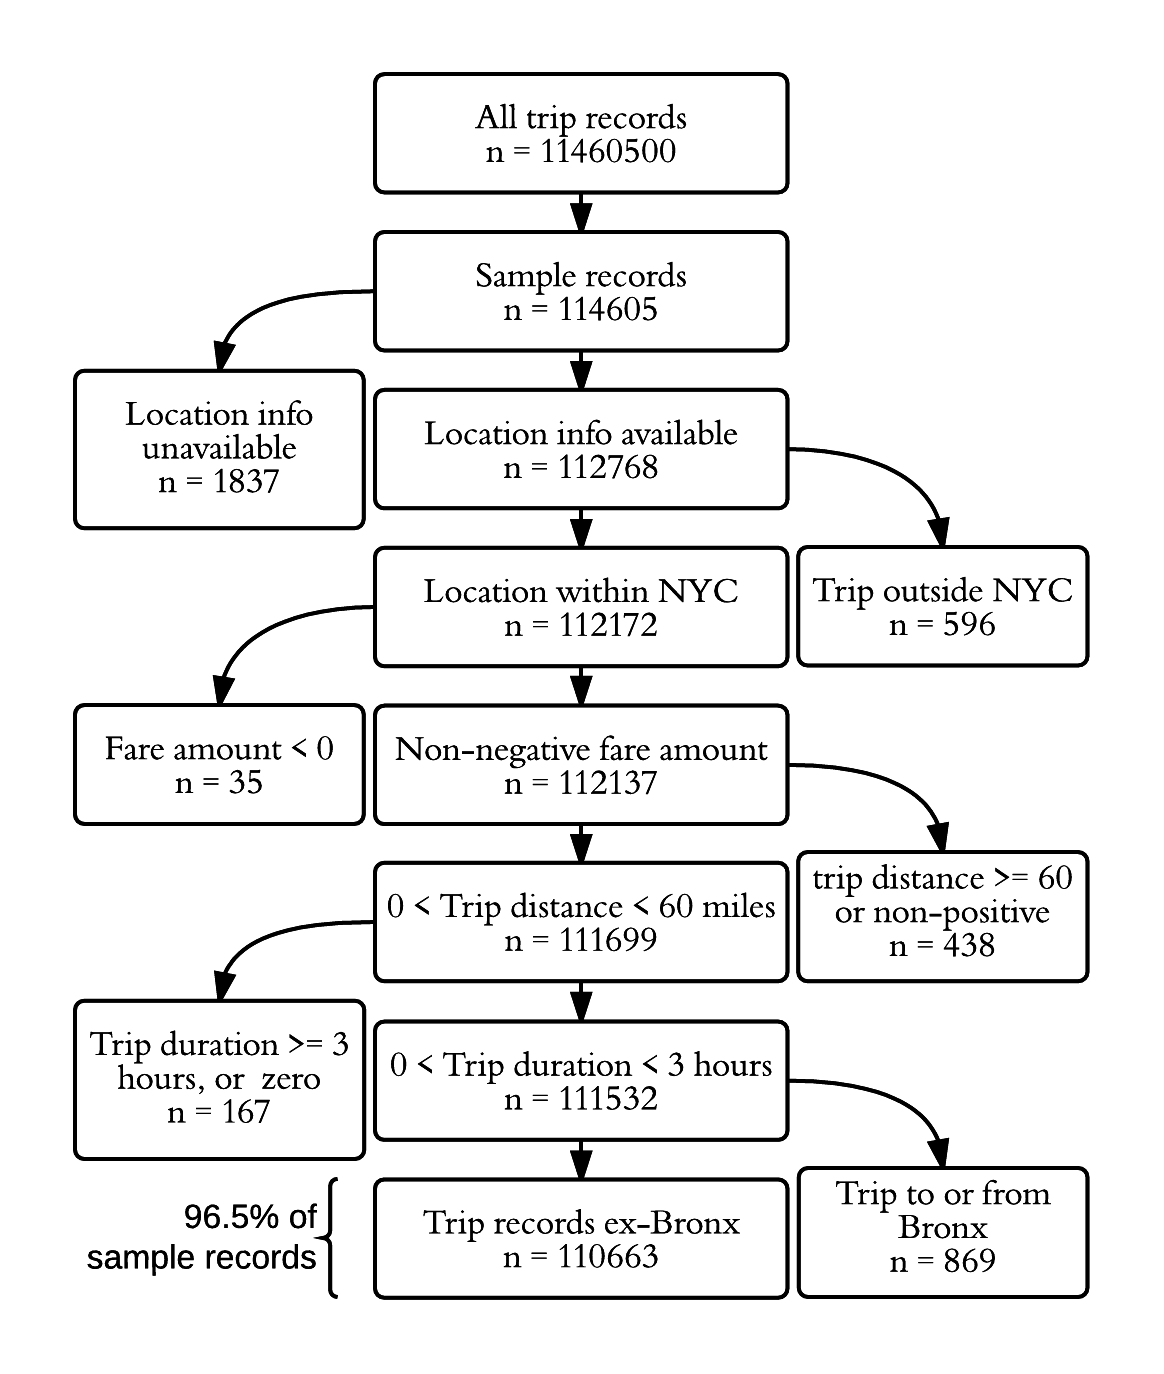
\includegraphics[width=8cm]{consort_diagram.png}
    %\caption{Consort diagram}\label{wrap-fig:1}
    %\end{wrapfigure} 

    %------------------------------------------
    {The New York City Taxi and Limousine Commission has made taxi trip records public and available in 2015\footnote{http://www.nyc.gov/html/tlc/html/about/trip\_record\_data.shtml}. The data set includes trip records from all trips completed in yellow and green taxis in NYC in 2014 and select months of 2015. Records include fields capturing pick-up and drop-off dates/times, pick-up and drop-off locations, trip distances, itemized fares, rate types, payment types, and driver-reported passenger counts. 
    We focus our attention on the yellow cab data collected in the month of December 2015.
    
    The data set consists of over 11 million entries of trip records, roughly 1.7 GB in disk volume. The data is of the `long' format (as opposed to the `fat' format), in which the number of covariates is small compared to the number of observations. Some subsampling is required for the data set to be handled on an average personal computer. Because $n$ is much larger than $p$ in this case, we do not expect to sacrifice much inferential quality in the sampling process. All subsequent analysis is based on a bootstrapped sample that is a random subset of size 1-percent of the the original records.
    
    There are abnormal data values and suspect entry errors noted in the data set, including wrong record of trip pick-up/drop-off locations, trip durations, trip distances, etc..  Only trip records within the city of New York is selected (ex-Staten Island and Bronx). We end up with about 95.6\% of the sampled data. The data cleaning and selection process in summarized in Figure \ref{fig:consort}.
    
    \begin{figure}
    \centering
    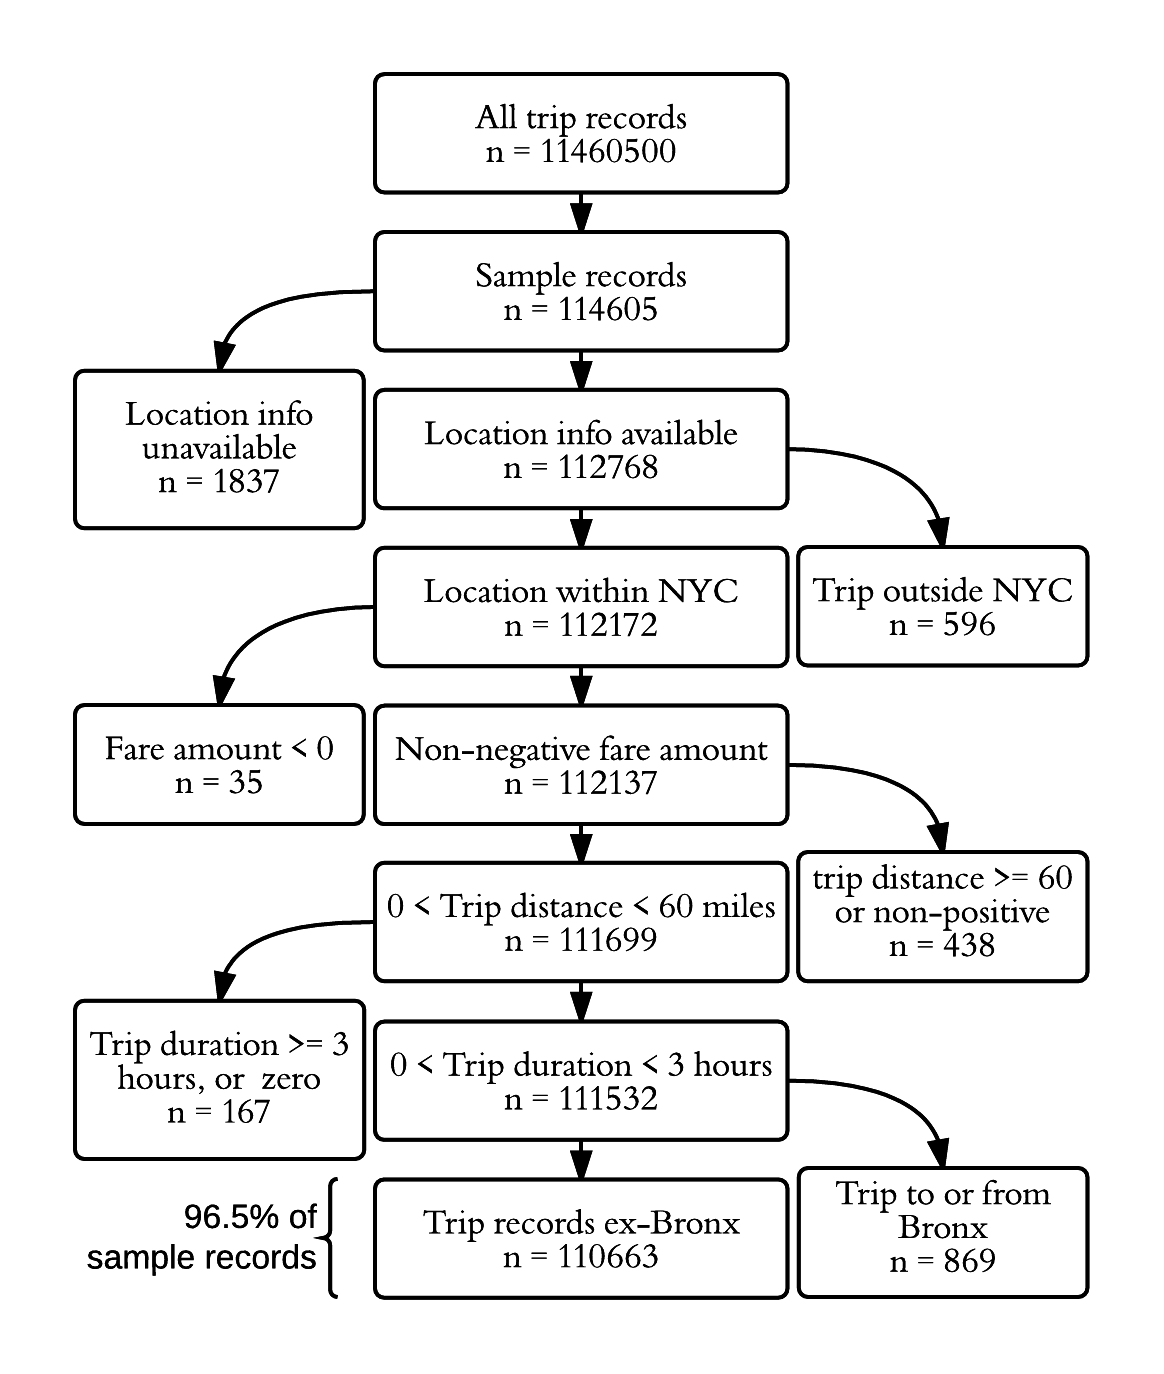
\includegraphics[width=0.5\linewidth]{consort_diagram.png}
    \caption{Consort diagram}\label{fig:consort}
    \end{figure} 
    
    
    %\par
    
    
    \section{Exploratory data analysis}
    
    Visualization helps revealing questions to be asked. Before endeavouring into the questions that one might be interested in, it is also important to understand which questions \emph{can} be answered, and where limitations lie.
    
    Some exploratory plots are in order.
    
    \subsection{Temporal patterns}
    
    How does Trip durations vary against pick-up time? Figure \ref{fig:trip-by-dayhours} (a) shows boxplots of Trip duration by hours and days of the week. Distributions of trip durations look roughly constant throughout the week, with dips on the weekend during day times. It is not clear whether this is due to a decrease in trip speed, a decrease in travel distance, or a combination of both. Let's look at trip distances.
    
    Figure \ref{fig:trip-by-dayhours} (b) shows boxplots of Trip distances by hours and days of the week. Trip distances tend to be longer at late nights and in early mornings, while being roughly constant throughout the day. How does travel speed look?
    
    Figure \ref{fig:trip-by-dayhours} (c) shows boxplots of Trip speed by hours and days of the week. Intriguing patterns emerge.
    Travel speed is higher at late nights 1 to 4am, increasing through early morning, starts to drop only at 8am. Even when speed has tapered off, 9am speed still seems higher than the rest of the day.
    In contrast to conventional wisdom that peak hour (630 - 930am) is the most busy period on the road, traffic condition does not seem to improve past 10am in the city of New York. \\
    
    \begin{figure}
    \centering
        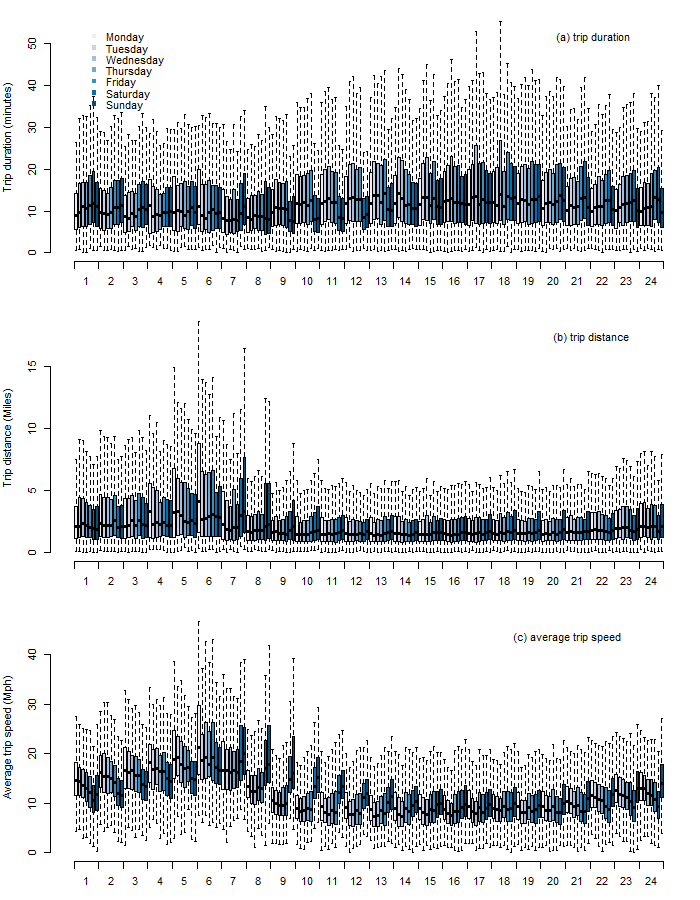
\includegraphics[width=\linewidth]{daily-hourly.png}
        \captionof{figure}{\textbf{(a) Trip duration, (b) distance, and (c) speed by hours and days of the week.} While trip durations are roughly uniform throughout the day and week, the trip distances are more variable, showing long distance travelling around morning hours. Speed, ratio of the trip distance by duration, shows an interesting pattern: average trip speed is higher in the morning hours than in the rest of the day. Is travelling in the morning actually faster, and morning rush hour only a myth?}
        \label{fig:trip-by-dayhours}
    \end{figure}
    
    Someone skeptical as statisticians starts to question the validity of the above finding. Alternative explanations abound. Could the Simpson's paradox be at play? More travellers are make long distance trips to work in the morning, taking highways or driving through areas with light traffic, inflating the average speed. Table \ref{table:simpsons} shows such a situation where the reported average speed in higher in the morning when in fact morning traffic is slower. 
    
    \begin{table}
    \begin{center}
        \begin{tabular}{ c  c  c }
            \hline
            \textbf{Time of the day} & \textbf{\# of long dist. traveller}  & \textbf{\# of downtown traveller} \\ \hline
            Morning         & 80 (at 40mph)     & 20 (at 10mph)\\ \hline
            Noon            & 20 (at 50mph)     & 80 (at 20mph)\\
            \hline
        \end{tabular}
        \caption{A hypothetical situation where reported average trip speed is higher in the morning. Average speed is 34mph in the morning and 26mph at noon, while in fact both type of travel are \emph{slower} in the morning.}
        \label{table:simpsons}
    \end{center}
    \end{table}
    
    Further investigations are needed.
    
    \subsection{Spatial patterns}
    
    With geographical data available, we can map out the pick up and drop off locations of the taxi rides.
    Figure \ref{fig:trip-by-pudo} upper panels show the pick up and drop off locations of trip colored by the neighborhood of the starting positions. Neighborhoods are defined approximately (and artificially) and not according to strict standards. The neighbourhood names are Upper Manhattan, Upper West, Upper East, Midtown, Downtown, Brooklyn Heights, North Brooklyn, East Queens, LaGuadia, and JFK Airport. Some natural clustering of destinations by origin neighborhood is evident. Trips within the same neighborhood, and by extension, short trips seem to be more common than long distance trips.
    
    Figure \ref{fig:trip-by-pudo} lower panels show the pick up and drop off locations of trip colored by the neighborhood of the destination positions. Similar clustering pattern appear. It may be easier to see that trips ending neighborhood mostly originates from the same neighborhood.\\
    

        
    \begin{figure}
    \centering
        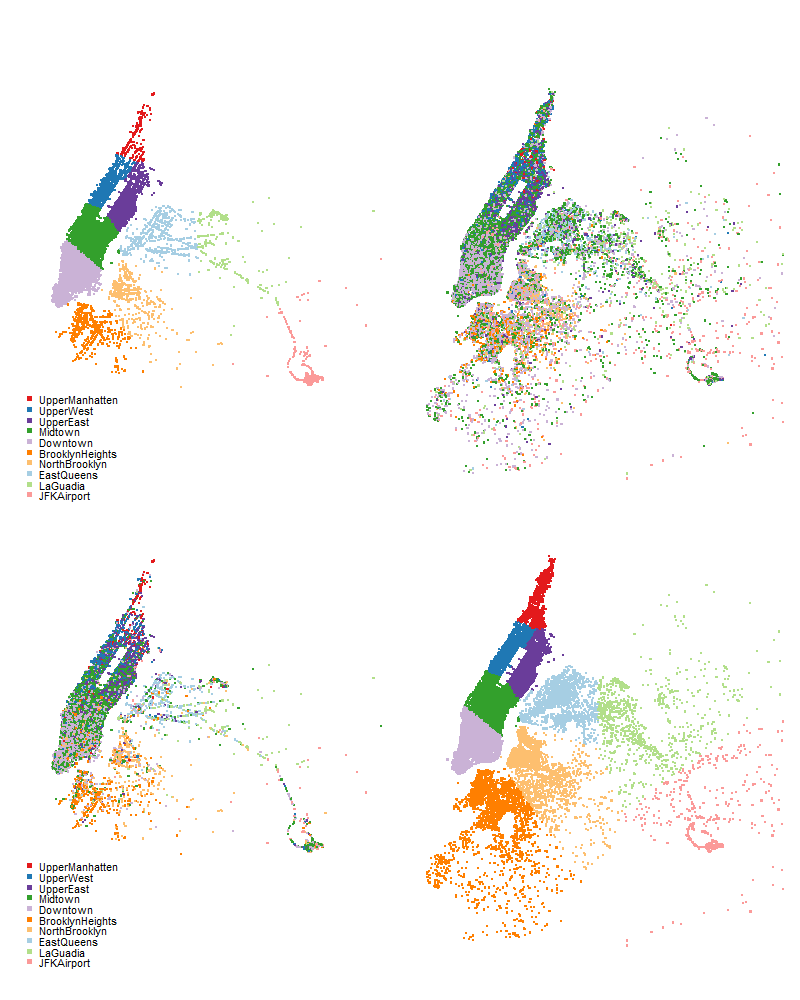
\includegraphics[width=\linewidth]{trip_by_pudo.png}
        \captionof{figure}{\textbf{Pick up (upper left) and drop off (upper right) locations, colored by pick up neighborhood.} And \textbf{pick up (lower left) and drop off (lower right) locations, colored by drop-off neighborhood.} Trip destinations tend to be near the pick up locations.}
        \label{fig:trip-by-pudo}
    \end{figure}
    
    
    With the geographical partition, we can look at trip information by the origin/destination combinations.
    Figure \ref{fig:trip-by-ori-dest} (a) shows a heat map of the trip distances by trip route, with red (by convention, signalling bad things) indicating further trips and blue (blue is like green, and green is good) denoting short-distance trips. Placing the nearby neighborhoods next to each other, the heat map shows a rather pleasing diagonal pattern. JFK airport is far away from almost all other neighborhoods.
    
    Figure \ref{fig:trip-by-ori-dest} (b) shows a heat map of the trip durations by trip route, with red indicating longer trips and blue denoting short trips. The trip durations is strongly positively correlated with the trip distances in panel (a).
    
    Figure \ref{fig:trip-by-ori-dest} (c) shows a heat map of the average trip speed by trip route, with red indicating slower trips and green denoting faster trips. Panel (c) tells a more interesting story: Trips to/from nearby neighborhoods tend to be slower on average, with downtown and midtown area being the slowest to travel in. Panel (c) together with panel (a) also reveals that short-distance trips tend to be slower in terms of speed. A possible explanation is that longer trips usually take highways and stop less for traffic lights, although is also possible that this marginal relationship breaks down when controlled for other factors.
    
    \begin{figure}
    \centering
        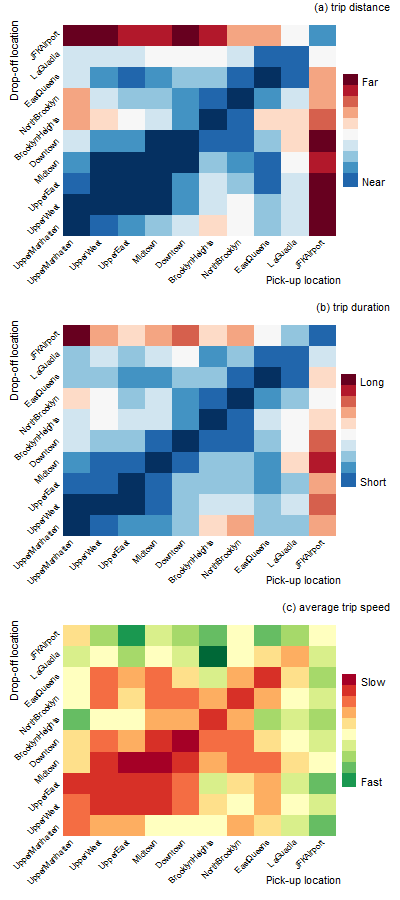
\includegraphics[height=0.7\textheight]{trip_by_ori_dest.png}
        \captionof{figure}{\textbf{(a) trip distance, (b) duration, and (c) speed by pick up and drop off neighborhood combinations.} Distance and duration are strongly correlated with each other. However, interesting patterns emerge when taking the ratio, i.e. speed. Trips that end up in nearby neighbourhoods tend to be slower than those travelling to places further away. Taxi rides to/from JFK airport, being the furthest trips to the rest of the neighbourhoods, actually enjoys the fastest travel speed.}
        \label{fig:trip-by-ori-dest}
    \end{figure}
    

    
    %\begin{wrapfigure}{r}{8cm}
    %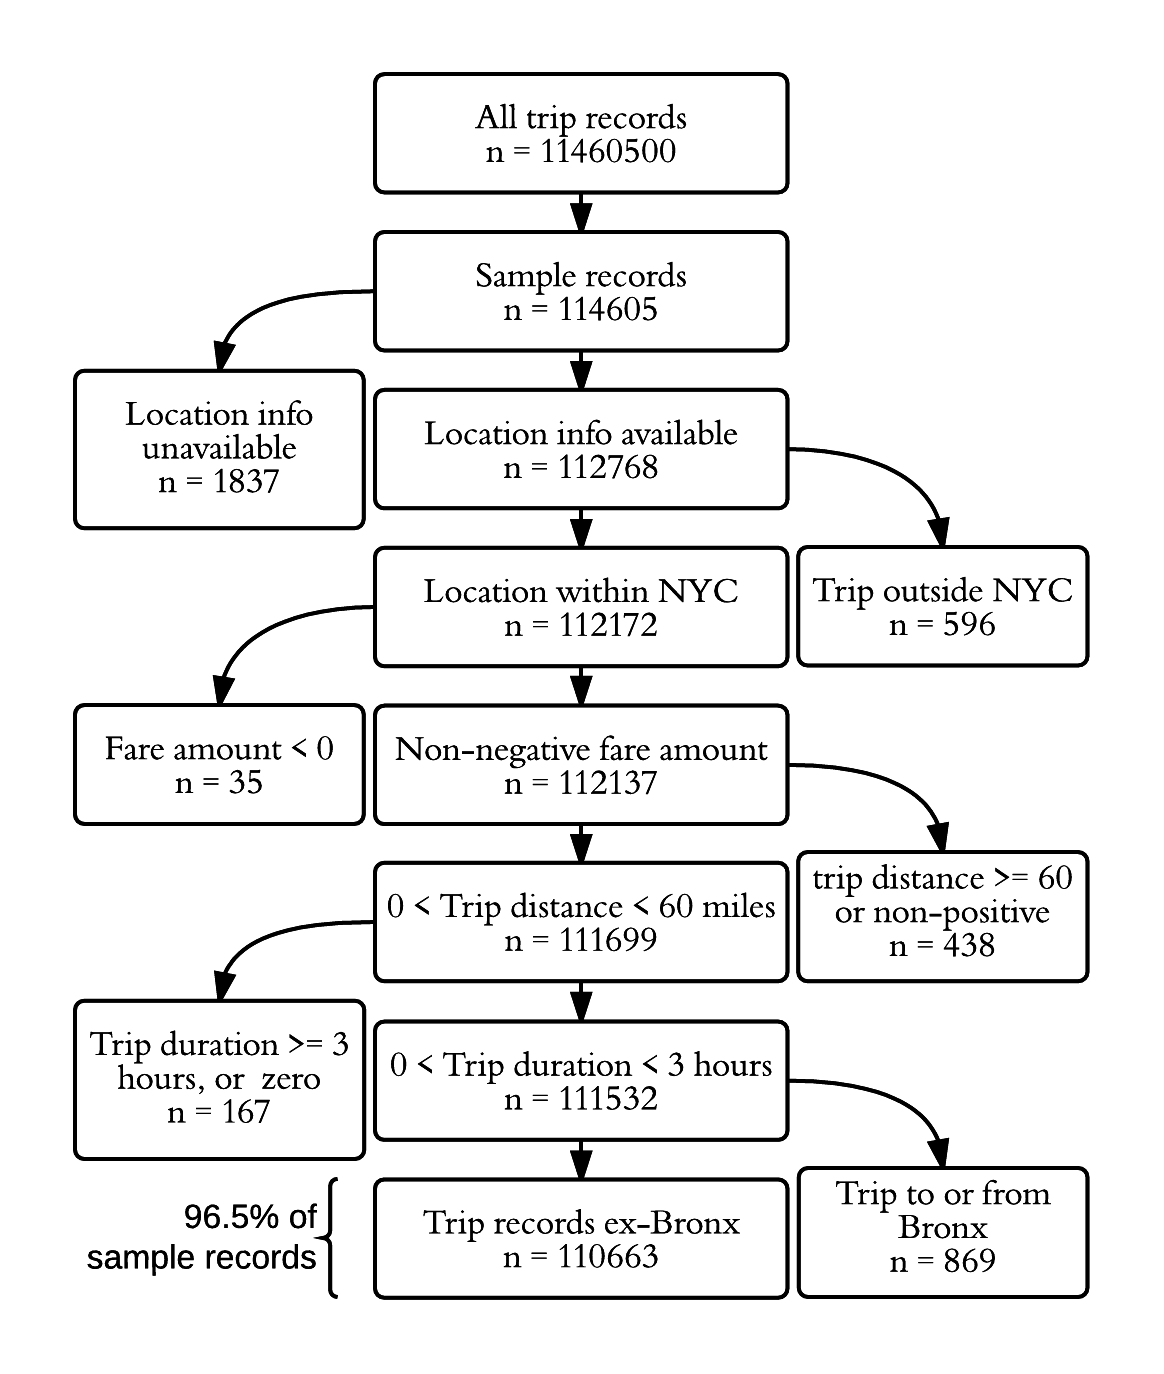
\includegraphics[width=8cm]{consort_diagram.png}
    %\caption{Consort diagram}\label{wrap-fig:1}
    %\end{wrapfigure} 
    

    \section{Modelling trip speed}
    
    \begin{wrapfigure}{r}{5cm}
        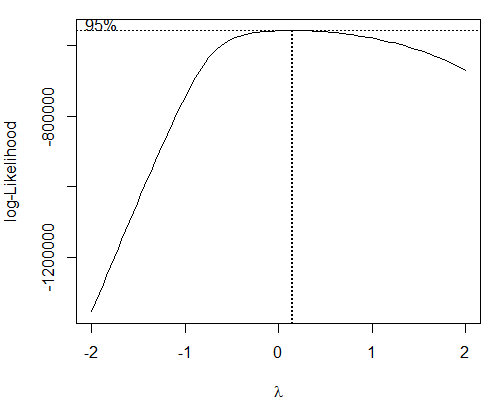
\includegraphics[width=5cm]{boxcox.png}
        \captionof{figure}{\textbf{Selection of Box-Cox transformation parameter.} Optimal $\lambda$ is $0.14$, with $0$ not far away. We choose the log-transformation (corresponding to $\lambda=0$) for easier interpretation without too much sacrifice on the variance stabilization front.}
        \label{fig:boxcox}
    \end{wrapfigure}
    
    As explored in the precious section, we would like to know if travel speed is indeed fast in the morning, hence busting the myth of morning `rush hours' in NYC, or could it be situations similar to a Simpson's paradox, where long distance travellers inflate the travel speed, masking the slower morning traffic.\\
    
    We shall first stabilize the variances using Box-Cox transformation, then model transformed travel speed against time. An argument for the methods used to control for routes will be made before we try to control for the confounding variables.
    
    \subsection{Variance stabilization}
    
    Box-Cox transformation is used for variance stabilization in the response variable. Likelihood peaks at around $0$ (see Figure \ref{fig:boxcox}). While the optimal is found to be $0.1414$, log-transformations (corresponding to Box-Cox transformation with $\lambda=0$) are much easier to interpret, and transformed data are off in terms of variance by less than $2\%$. We will continue with the log-transformed trip speed in modelling.
    
    %\begin{figure}
    %\centering
    %    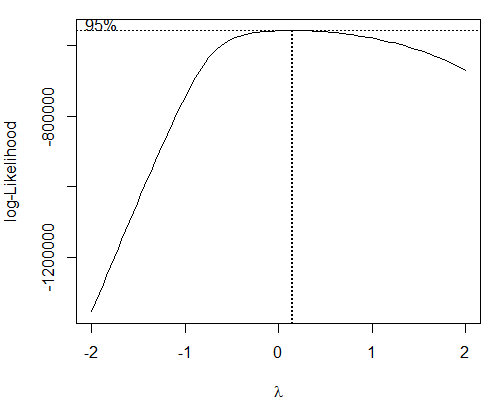
\includegraphics[width=4.5cm]{boxcox.png}
    %    \captionof{figure}{\textbf{Selection of Box-Cox transformation parameter.} Optimal $\lambda$ is $0.14$, with $0$ not far away. We choose the log-transformation (corresponding to $\lambda=0$) for easier interpretation without too much sacrifice on the variance stabilization front.}
    %    \label{fig:boxcox}
    %\end{figure}
    
    
    \subsection{Model selection}
    
    Model selection is based on BIC values.\\We compare the following three models $$log(\mathrm{Speed})\sim\mathrm{Day\ of\ the\ week}$$ $$log(\mathrm{Speed})\sim\mathrm{Weekdays + Weekends}$$ $$log(\mathrm{Speed})\sim\mathrm{Weekdays + Saturdays + Sundays}$$\\
    BIC values are 167831.5, 168669, 168132.2, respectively, and indicate clear preference for the full model. We will build upon that.
    
    Adding in the time-of-the-day component, we compare a model with and without interaction between day of the week and time of the day. $$log(\mathrm{Speed})\sim\mathrm{Day\ of\ the\ week}*\mathrm{pickup\ time}$$ $$log(\mathrm{Speed})\sim\mathrm{Day\ of\ the\ week}+\mathrm{pickup\ time}$$ where `$*$' denotes the inclusion of interaction terms. BIC value for the former is 148474.4, with the latter giving us 152109. We choose to model the speed with the full interaction model.
    
    Figure \ref{fig:boxcoxfit} shows the fitted values of model, overlaid on the actual data.
    
    \begin{figure}
    \centering
        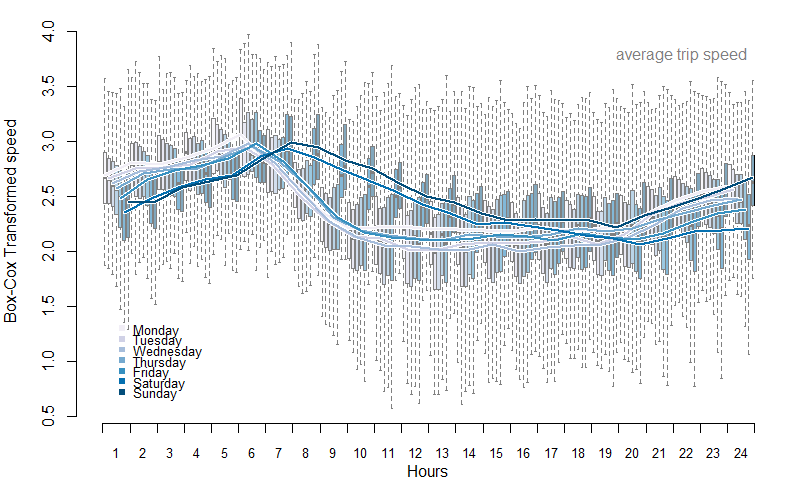
\includegraphics[width=\linewidth]{boxcoxfit.png}
        \captionof{figure}{\textbf{Fitted model of log-transformed average trip speed.} Model selection indicates strong interaction between day of the week and time of the day. Each curves represents the fitted values of travel speed throughout the day by the day of the week. Travel speed peaks at early morning 6am and bottoms out from 10am to 7pm daily on weekdays. No sign of the usual ``rush hour'' (630 - 930am) is present. Notably, vehicles travel slower on Friday and Saturday nights, while Sunday nights enjoy smoother rides. Cars cruise at a higher speed on Saturday and Sunday mornings.}
        \label{fig:boxcoxfit}
    \end{figure}
    
    
    \subsection{Model diagnostics}
    
    \begin{figure}
    \centering
        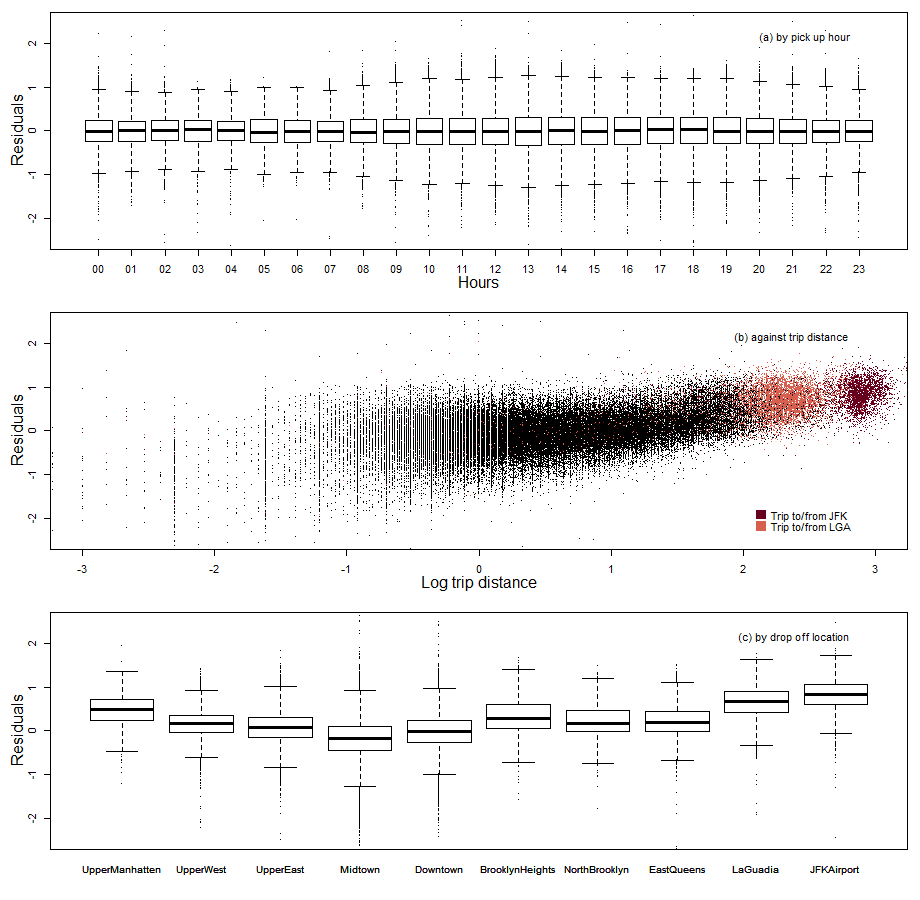
\includegraphics[width=\linewidth]{residualModel1.png}
        \captionof{figure}{\textbf{Residual of Naive model against (a) pick up hours, (b) log transformed trip distance, and (c) drop off locations.} Residuals are roughly stable against trip starting time. Plot of residuals against distance in (b) indicates a positive correlation, a signal that trip distance should be adjusted for. Drop-off locations are also correlated with the residual terms, with Manhattan area showing slow downs and airports being the fastest destinations in terms of speed. In particular, trips to and from the airports are also the longest in distance and have mostly positive residuals.}
        \label{fig:residual1}
    \end{figure}
    
    
    Figure \ref{fig:residual1} shows the model diagnostic plots for the selected model.
    
    Panel (a) shows residuals against trip starting time. variances are roughly stable and slow varying.  Plot of residuals against distance in (b) indicates a positive correlation, a signal that trip distance should be adjusted for. Drop-off locations are also correlated with the residual terms.
    
    
    \section{Controlling for trip routes}
    
    In an \emph{ideal} situation we would be able to tell if morning traffic is slower should we know all the routes of the trips. Controlling for the routes would be simply to extract identical routes: direct comparison can be made about trip speed for the same routes at different trip pick up times. 
    
    With only the currently published data available, we are not able to know the exact streets and avenues the drivers decided to take, but only the starting and end points and distances of the trip. As a proxy, we can use the \textbf{pick-up location}, \textbf{drop-off location}, and \textbf{trip distance} to control for trip routes, in the hope that trips with similar attributes in these variables have taken similar routes, making them comparable.
    
    \subsection{Adding trip distance to the model}
    
    Residual plot indicates linear relationship of speed and distance in log-log level. BIC value of the following model is $106652.9$, indicating significant improvement of fit.
    $$log(\mathrm{Speed})\sim\mathrm{Day\ of\ the\ week}*\mathrm{pickup\ time} + log(\mathrm{trip\ distance})$$
    
    \subsection{Adding trip origin / destination to the model}
    
    we compare a model with and without interaction between the origin and destinations.
    \begin{multline}
        log(\mathrm{Speed})\sim\mathrm{Day\ of\ the\ week}*\mathrm{pickup\ time} +\\ + log(\mathrm{trip\ distance}) + \mathrm{pick\ up\ neighborhood} + \mathrm{drop\ off\ neighborhood}
    \end{multline}
    \begin{multline}
        log(\mathrm{Speed})\sim\mathrm{Day\ of\ the\ week}*\mathrm{pickup\ time} +\\ + log(\mathrm{trip\ distance}) + \mathrm{pick\ up\ neighborhood} * \mathrm{drop\ off\ neighborhood}
    \end{multline}
    with (1) giving BIC value $90763.39$ and (2) giving a smaller $89683.83$. We select the model with full interaction terms, i.e., with $10$ factor levels for both pick up and drop off locations, a total of $100$ combinations of trip routes are controlled for.
    
    Again we look at diagnostic plots (Figure \ref{fig:residual2}): Troubling features in the residual plots of the Naive model are gone. Distributions of residuals across different trip distances and at different levels of trip destinations are roughly the same, with no sign of trend or variations in standard deviations.\\
    
    \begin{figure}
    \centering
        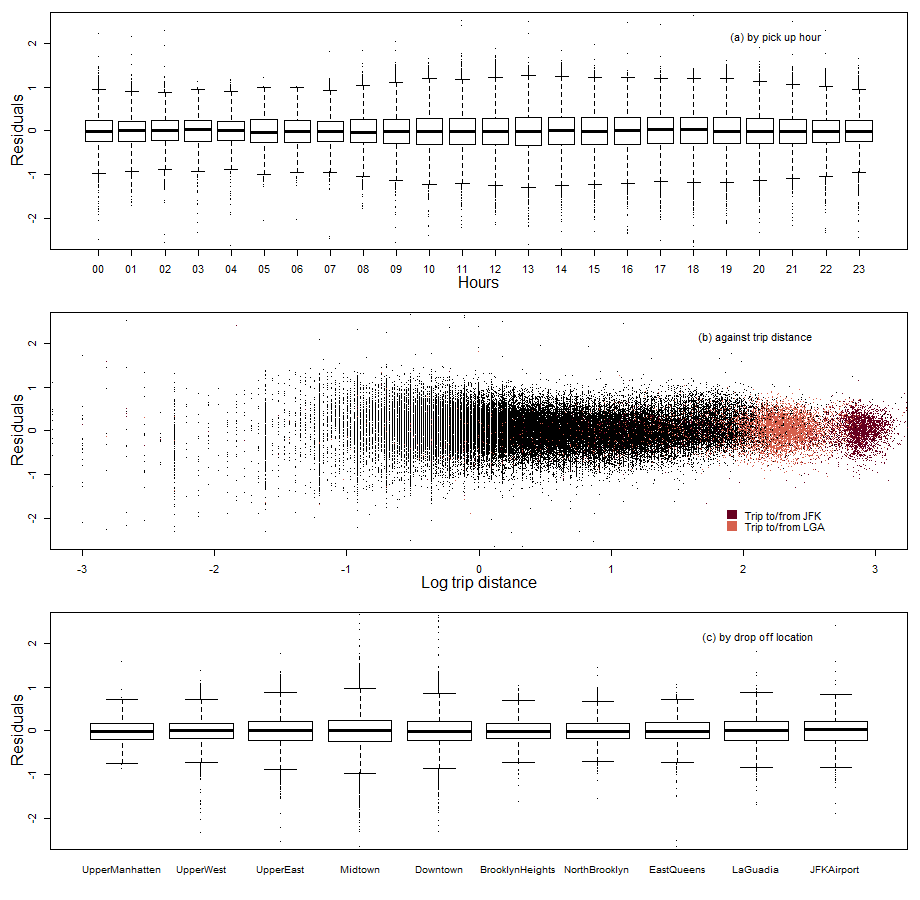
\includegraphics[width=\linewidth]{residualModel2.png}
        \captionof{figure}{\textbf{Residual of the Full model against (a) pick up hours, (b) log transformed trip distance, and (c) drop off locations.} Previous troubling features in (b) are gone: distances are no longer positively correlated with residuals, variances are roughly constant across different values of trip distances. Drop-off locations are also uncorrelated with residuals. Some unevenness in the standard deviation of residuals against drop off location is noted.}
        \label{fig:residual2}
    \end{figure}
    
    \section{Interpretations and further discussions}
    
    The final `Full' model is easy to interpret: for a certain trip origin/destination combination, fixing the travel distance, time effect can be plotted against the hours for any day of the week. See Figure \ref{fig:effect}. For example, the same trip would be on average $\mathrm{exp}\{0.06764552-(-0.42742022)\}=1.64$ times faster at Monday $6$am vs Monday $12$noon, while the Naive model would predict a speed that is $\mathrm{exp}\{0.12298178-(-0.49217586)\}=1.85$ times faster.\\
    
    Notice that part of the `time effect' in the Naive model gets adjusted for the trip routes in the Full model. Adjusted time effect is dampened in the Full model, reflecting the fact that longer-distance (and high-speed) trips increase in proportion during the late night and early morning hours, and inflating the average speed. While during the day, shorter distance travels dominate, and make average trip speed appear slower than they actually are.\\
    
    There are no signs of dipping pattern around $630$ - $930$am in the adjusted time effects. Travel speed remain low throughout the day from $10$am to around $7$pm. New York City traffic does not get any easier after so-called `rush hours'.\\
    
    \begin{figure}
    \centering
        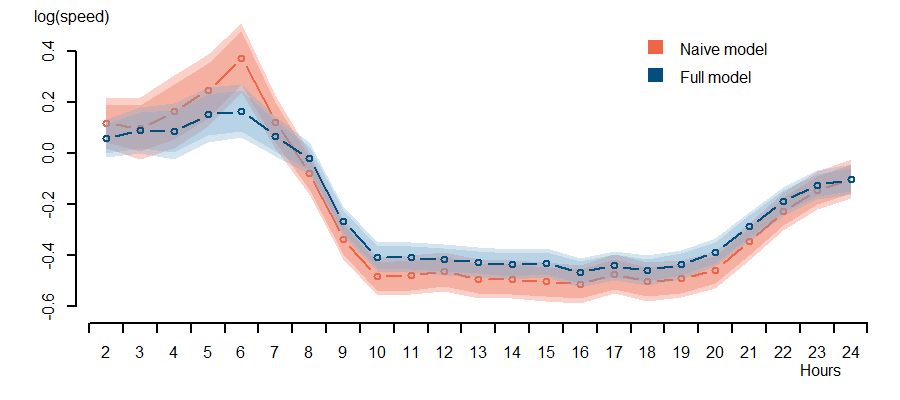
\includegraphics[width=\linewidth]{effect.png}
        \captionof{figure}{\textbf{Time effect (Monday) on trip speed of Naive model, vs Full model adjusted for trip routes.} The full model accounts for the trip routes, with pick-up, drop-off locations, and distances as proxies. Part of the speed difference is attributed to the route differences under the full model, as we expected in exploratory data analysis. The travel speed is still faster in the morning and slow throughout the day. No `rush hour' pattern was found even after the adjustments.}
        \label{fig:effect}
    \end{figure}
    
    \section{Improvements and limitations}
    
    improvements to the current model can be achieved through a finer geographical definition of neighborhoods of the trip origin/destinations. Utilization of intermediate GPS location information during a trip might enable us to refine the trip routes categories. The idea of controlling for the trip routes is the same.
    
    One might also consider interactions between trip routes and time. Since not all trips are affected the same way: speed of a trip from Downtown to Midtown may vary greatly by the hour, but a trip from Brooklyn Heights to Williamsburg may not vary as much, even after adjusting for trip routes.\\
    
    Limitation of the current model and above improvements is clear: even if all routes are known exactly, controlling for the routes would be extremely difficult, since two routes are different levels if they differ by just a single turn at one crossroad, resulting in an astronomical number of routes. Problem quickly gets out of hand. One might want to devise smarter ways to control for travel routes: segmenting the trip into street blocks and piecing them together may be a better solution.\\
    
    
    Source code and output of this project can be found at:\\ \url{https://github.com/Pill-GZ/QRDataAnalysis}.

    %\par
    
    % bib stuff
    \nocite{*}
    \addtocontents{toc}{\protect\vspace{\beforebibskip}}
    \addcontentsline{toc}{section}{\refname}    
    \bibliographystyle{plain}
    \bibliography{../Bibliography}
    %\finalVersionString
\end{document}
%